\documentclass[french]{article}
\usepackage[T1]{fontenc}
\usepackage[utf8]{inputenc}
\usepackage{lmodern}
\usepackage[a4paper]{geometry}
\usepackage{babel}
\usepackage{amsmath}
\usepackage{amsfonts}
\usepackage{tcolorbox}
\usepackage{color}
\usepackage{breqn}
\usepackage{tcolorbox}

\usepackage{tikz}
\usetikzlibrary{arrows,shapes}

\begin{document}
	\title{DM: Chaînes de Markov (Comportement asymptotique)}
	\author{Gabriel PEREIRA DE CARVALHO}
	\date{Dernière modification \today}
	
	\maketitle
	
	\section*{Exercice 1: Deux variantes de l'algorithme de Metropolis-Hastings}
	
	\subsection*{Algorithme de Metropolis-Hastings}
	
	\begin{tcolorbox}[colback=gray!5!white,colframe=gray!75!black]
		\textbf{1.} Exprimer la matrice de transition de la chaîne de Markov $(X_n)_{n \geq 0}$ en fonction de $\pi$ et $Q$. En déduire que la chaîne de Markov est irréductible.
	\end{tcolorbox}
	
	Soit $R: (x,y) \in E^2 \mapsto \min\left\{1, \frac{\pi(y) Q(y,x)}{\pi(x) Q(x,y)} \right\}$ la probabilité d'acceptation.
	
	Alors, $\forall y \not= X_n$ on a $X_{n+1} = y$ avec probabilité $Q(X_n, y)R(X_n, y)$ car les tirages de $\tilde{X}_{n+1}$ et $U_{n+1}$ sont indépendantes. Donc, soit $P$ la matrice de transition, on a
	
	\begin{align}
		\begin{cases}
		P(x, y) &= Q(x,y)R(x,y) \qquad \forall y \not=x \\
		P(x, x) &= 1 - \sum_{y \not= x} P(x,y)
		\end{cases}
	\end{align}
		
	 Alors, on remarque que $Q$ irréductible sur $E \implies P$ irréductible sur $E$. 
	
	\begin{tcolorbox}[colback=gray!5!white,colframe=gray!75!black]
		\textbf{2.} Montrer que $(X_n)_{n \geq 0}$ est réversible par rapport à $\pi$.
	\end{tcolorbox}

	Premièrement, on remarque que $\frac{R(x,y)}{R(y,x)} = \frac{\min\left\{1, \frac{\pi(y) Q(y,x)}{\pi(x) Q(x,y)} \right\}}{\min\left\{1, \frac{1}{\frac{\pi(y) Q(y,x)}{\pi(x) Q(x,y)}} \right\}}  = \frac{\pi(y) Q(y,x)}{\pi(x) Q(x, y)}$.

	Montrons que
	
	$$\forall x,y \in E, \qquad \pi(x)P(x,y) = \pi(y)P(y,x)$$
	
	Pour $x=y$ c'est vrai. Alors, supposons $x \not= y$.
	
	On calcule
	
	\begin{align}
		\frac{\pi(x)P(x,y)}{\pi(y)P(y,x)} &= \frac{\pi(x)Q(x,y)R(x,y)}{\pi(y)Q(y,x)R(y,x)} \\
		&= \frac{\pi(x)Q(x,y)}{\pi(y)Q(y,x)} \frac{\pi(y) Q(y,x)}{\pi(x) Q(x, y)} \\
		&= 1.
	\end{align}
	
	On en conclue que $(X_n)_{n \geq 0}$ est réversible par rapport à $\pi$.

	\begin{tcolorbox}[colback=gray!5!white,colframe=gray!75!black]
		\textbf{3.} En déduire un résultat de convergence des moyennes trajectorielles.
	\end{tcolorbox}

	Soit $F: E \to \mathbb{R}$ tel que $\mathbb{E}_{\pi}(|F|) < \infty$. Soit $X_0 \in E$ la donnée initiale de la trajectoire.
	
	On remarque que la chaîne de Markov	$(X_n)_{n \geq 0}$ avec matrice de transition $P$ est irréductible avec mesure invariante unique $\pi$. Donc, par le \textbf{Théorème ergodique}, les moyennes  trajectorielles convergent presque sûrement,
	
	$$ \frac{1}{n} \sum_{i=0}^{n-1} F(X_i)  \xrightarrow[]{n \to +\infty} \mathbb{E}_{\pi}(F) $$	
	
	\subsection*{Première variante}
	
	\begin{tcolorbox}[colback=gray!5!white,colframe=gray!75!black]
		\textbf{1.} Exprimer la matrice de transition de la chaîne de Markov $(X_n)_{n \geq 0}$ en fonction de $\pi$ et $Q_1, Q_2$. En déduire que la chaîne de Markov est irréductible.
	\end{tcolorbox}

	Soit $R: (x,y,z) \in E^3 \mapsto \min\left\{1, \frac{\pi(z) Q_1(z,y) Q_2(y, x)}{\pi(x) Q_1(x,y) Q_2(y,z)} \right\}$ la probabilité d'acceptation.
	
	Alors, $\forall z \not= X_n$ on a $X_{n+1} = z$ avec probabilité $\sum_{y \in E} Q_1(x, y) Q_2(y, z) R(x,y,z)$.
	
	Donc, soit $P$ la matrice de transition, on a
	
	\begin{align}
	\begin{cases}
	P(x, z) &= \sum_{y \in E} Q_1(x, y) Q_2(y, z) R(x,y,z) \qquad \forall z \not=x \\
	P(x, x) &= 1 - \sum_{z \not= x} P(x,z)
	\end{cases}
	\end{align}
	
	Alors, on remarque que $Q_1, Q_2$ irréductible sur $E \implies P$ irréductible sur $E$. 

	\begin{tcolorbox}[colback=gray!5!white,colframe=gray!75!black]
		\textbf{2.} Montrer que $(X_n)_{n \geq 0}$ est réversible par rapport à $\pi$.
	\end{tcolorbox}

	Premièrement, on remarque que $\frac{R(x,y,z)}{R(y,x,z)} = \frac{\min\left\{1, \frac{\pi(z) Q_1(z,y) Q_2(y, x)}{\pi(x) Q_1(x,y) Q_2(y,z)} \right\}}{\min\left\{1, \frac{1}{\frac{\pi(z) Q_1(z,y) Q_2(y, x)}{\pi(x) Q_1(x,y) Q_2(y,z)}} \right\}}  = \frac{\pi(z) Q_1(z,y) Q_2(y, x)}{\pi(x) Q_1(x,y) Q_2(y,z)}$.
	
	Montrons que
	
	$$\forall x,z \in E, \qquad \pi(x)P(x,z) = \pi(z)P(z,x)$$
	
	Pour $x=z$ c'est vrai. Alors, supposons $x \not= z$.
	
	On calcule
	
	\begin{align}
	\frac{\pi(x)P(x,z)}{\pi(z)P(z,x)} &= \frac{\pi(x) \sum_{y \in E} Q_1(x, y) Q_2(y, z) R(x,y,z)}{\pi(z) \sum_{y \in E} Q_1(z, y) Q_2(y, x) R(z,y,x)} \\
	&= \frac{\sum_{y \in E} \pi(x) Q_1(x, y) Q_2(y, z) R(z,y,x) \frac{\pi(z) Q_1(z,y) Q_2(y, x)}{\pi(x) Q_1(x,y) Q_2(y,z)}}{\sum_{y \in E} \pi(z) Q_1(z, y) Q_2(y, x) R(z,y,x)} \\
	&= \frac{\sum_{y \in E} \pi(z) Q_1(z,y) Q_2(y, x) R(z,y,x)}{\sum_{y \in E} \pi(z) Q_1(z, y) Q_2(y, x) R(z,y,x)}\\
	&= 1.
	\end{align}
	
	On en conclue que $(X_n)_{n \geq 0}$ est réversible par rapport à $\pi$.

	\begin{tcolorbox}[colback=gray!5!white,colframe=gray!75!black]
		\textbf{3.} En déduire un résultat de convergence des moyennes trajectorielles.
	\end{tcolorbox}
	
	Soit $F: E \to \mathbb{R}$ tel que $\mathbb{E}_{\pi}(|F|) < \infty$. Soit $X_0 \in E$ la donnée initiale de la trajectoire.
	
	On remarque que la chaîne de Markov	$(X_n)_{n \geq 0}$ avec matrice de transition $P$ est irréductible avec mesure invariante unique $\pi$. Donc, par le \textbf{Théorème ergodique}, les moyennes  trajectorielles convergent presque sûrement,
	
	$$ \frac{1}{n} \sum_{i=0}^{n-1} F(X_i)  \xrightarrow[]{n \to +\infty} \mathbb{E}_{\pi}(F) $$	

	
	
	\subsection*{Deuxième variante}
	
	\begin{tcolorbox}[colback=gray!5!white,colframe=gray!75!black]
		\textbf{1.} Exprimer la matrice de transition de la chaîne de Markov $(X_n)_{n \geq 0}$ en fonction de $\pi$ et $Q_0, Q_1$. En déduire que la chaîne de Markov est irréductible.
	\end{tcolorbox}
	
	Soit $\forall c \in \{0,1\}, \quad  R_c: (x,y) \in E^2 \mapsto \min\left\{1, \frac{\pi(y) Q_{1-c}(y, x)}{\pi(x) Q_c(x,y)} \right\}$ la probabilité d'acceptation pour $C_{n+1} = c$.
	
	Alors, $\forall y \not= X_n$ on a $X_{n+1} = y$ avec probabilité $\frac{1}{2}Q_0(X_n, y)R_0(X_n, y) + \frac{1}{2}Q_1(X_n, y)R_1(X_n, y)$.
	
	Donc, soit $P$ la matrice de transition, on a
	
	\begin{align}
	\begin{cases}
	P(x, y) &= \frac{1}{2}Q_0(x, y)R_0(x, y) + \frac{1}{2}Q_1(x, y)R_1(x, y) \qquad \forall y \not=x \\
	P(x, x) &= 1 - \sum_{y \not= x} P(x,y)
	\end{cases}
	\end{align}
	
	Alors, on remarque que $Q_0, Q_1$ irréductible sur $E \implies P$ irréductible sur $E$. 
	
	\begin{tcolorbox}[colback=gray!5!white,colframe=gray!75!black]
		\textbf{2.} Montrer que $(X_n)_{n \geq 0}$ est réversible par rapport à $\pi$.
	\end{tcolorbox}

	Premièrement, $\forall c \in \{0,1\}$ ,on remarque que 
	\begin{align}
		\frac{R_c(x,y)}{R_{1-c}(y,x)} &= \frac{\min\left\{1, \frac{\pi(y) Q_{1-c}(y,x)}{\pi(x) Q_c(x,y)} \right\}}{\min\left\{1, \frac{\pi(x) Q_c(x,y)}{\pi(y) Q_{1-c}(y,x)} \right\}}\\
		&= \min\left\{1, \frac{\pi(y) Q_{1-c}(y,x)}{\pi(x) Q_c(x,y)} \right\} \max\left\{1, \frac{\pi(y) Q_{1-c}(y,x)}{\pi(x) Q_c(x,y)} \right\}\\
		&= \frac{\pi(y) Q_{1-c}(y,x)}{\pi(x) Q_c(x,y)}
	\end{align}
	
	Montrons que
	
	$$\forall x,y \in E, \qquad \pi(x)P(x,y) = \pi(y)P(y,x)$$
	
	Pour $x=y$ c'est vrai. Alors, supposons $x \not= y$.
	
	On calcule
	
	\begin{align}
	\frac{\pi(x)P(x,y)}{\pi(y)P(y,x)} &= \frac{\pi(x)\left(\frac{1}{2}Q_0(x,y)R_0(x,y) + \frac{1}{2}Q_1(x,y)R_1(x,y)\right)}{\pi(y)\left(\frac{1}{2}Q_0(y,x)R_0(y,x) + \frac{1}{2}Q_1(y,x)R_1(y,x)\right)} \\
	&= \frac{\pi(x)Q_0(x,y)R_0(x,y) + \pi(x)Q_1(x,y)R_1(x,y)}{\pi(y)Q_0(y,x)R_0(y,x) + \pi(y)Q_1(y,x)R_1(y,x)}\\
	&= \frac{\pi(x)Q_0(x,y)R_1(y,x)\frac{\pi(y) Q_1(y,x)}{\pi(x) Q_0(x, y)} + \pi(x)Q_1(x,y)R_0(y,x)\frac{\pi(y) Q_0(y,x)}{\pi(x) Q_1(x, y)}}{\pi(y)Q_0(y,x)R_0(y,x) + \pi(y)Q_1(y,x)R_1(y,x)} \\
	&= \frac{\pi(y)Q_1(y,x)R_1(y,x) + \pi(y)Q_0(y,x)R_0(y,x)}{\pi(y)Q_0(y,x)R_0(y,x) + \pi(y)Q_1(y,x)R_1(y,x)}\\
	&= 1.
	\end{align}
	
	On en conclue que $(X_n)_{n \geq 0}$ est réversible par rapport à $\pi$.
	
	\begin{tcolorbox}[colback=gray!5!white,colframe=gray!75!black]
		\textbf{3.} En déduire un résultat de convergence des moyennes trajectorielles.
	\end{tcolorbox}

	Soit $F: E \to \mathbb{R}$ tel que $\mathbb{E}_{\pi}(|F|) < \infty$. Soit $X_0 \in E$ la donnée initiale de la trajectoire.
	
	On remarque que la chaîne de Markov	$(X_n)_{n \geq 0}$ avec matrice de transition $P$ est irréductible avec mesure invariante unique $\pi$. Donc, par le \textbf{Théorème ergodique}, les moyennes  trajectorielles convergent presque sûrement,
	
	$$ \frac{1}{n} \sum_{i=0}^{n-1} F(X_i)  \xrightarrow[]{n \to +\infty} \mathbb{E}_{\pi}(F) $$
	
	
	\section*{Exercice 2: Couplage et critère de Doeblin}
	
	On vérifie que pour chaque $x_n$, l'expression donné définit une probabilité.
	
	Pour $n_0 = 1$, on a $\forall z \in E, \quad P(x,z) \geq \alpha m(z)$.
	
	D'où $\forall z \in E, \quad \frac{1}{1-\alpha}\left(P(x, z) - \alpha m(z)\right) \geq 0$.
	
	Alors, on calcule la somme des probabilités
	
	$$ \sum_{z \in E} \frac{1}{1-\alpha}\left(P(x, z) - \alpha m(z)\right) = \frac{1}{1 - \alpha} \sum_{z \in E} P(x, z) - \frac{\alpha}{1 - \alpha} \sum_{z \in E} m(z) = 1.$$
	
	\begin{tcolorbox}[colback=gray!5!white,colframe=gray!75!black]
		\textbf{0.} Trouver un exemple de chaîne de Markov apériodique, irréductible et récurrente positive qui ne vérifie pas (1).
	\end{tcolorbox}
	
	Considérons la chaîne de deux états avec matrice de transition $P = \begin{pmatrix}
	0,2 & 0,8 \\
	0,5 & 0,5
	\end{pmatrix}.$
	
	\begin{center}
		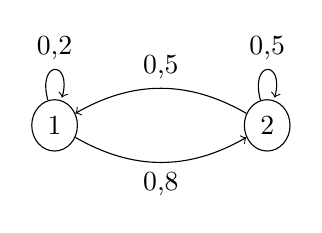
\begin{tikzpicture}[->]
		\node[ellipse,draw] (N) at (8.5,8.5) {1};
		\node[ellipse,draw] (Y) at (11.2,8.5) {2};     
		\path (N) edge [loop above] node {0,2} (N);
		\path (Y) edge [loop above] node {0,5} (Y);
		\path (N) edge [bend right] node[below] {0,8} (Y);
		\path (Y) edge [bend right] node[above] {0,5} (N);
		\end{tikzpicture}
	\end{center}

	On remarque que la chaîne est irréductible par connexité du graphe de transtions. 
	
	Par le \textbf{Théorème 4.6} du cours, on sait que cette chaîne est recurrente positive $\iff$ elle admet l'unique mesure invariante. On calcule
	\begin{align}
	\begin{cases}
		&0,2 \pi(1) + 0,5 \pi(2) = \pi(1)\\
		&0,8 \pi(1) + 0,5\pi(2) = \pi(2)\\
		&\pi(1) + \pi(2) = 1
	\end{cases}
	\iff \begin{cases}
	\pi(1) &= \frac{5}{13}\\
	\pi(2) &= \frac{8}{13}
	\end{cases}
	\end{align}

	donc, la chaîne est récurrente positive. Et la chaîne est apériodique car $$\forall x,y \in E, \quad \forall n \in \mathbb{N}, \quad P^n(x, y)>0.$$
	
	\begin{tcolorbox}[colback=gray!5!white,colframe=gray!75!black]
		\textbf{1.} Vérifier que P est la matrice de transition de la chaîne de Markov $(X_n)_{n \in \mathbb{N}}$.
	\end{tcolorbox}

	Calculons la probabilité de la transition $X_n \to z \in E$.
	
	Fixons $X_n = x$. On a 

	\begin{align*}
		\forall z \in E, \quad \mathbb{P}(X_{n+1} = z) &= \mathbb{P}(X_{n+1} = z| B_{n+1} = 0)\mathbb{P}(B_{n+1} = 0) + \mathbb{P}(X_{n+1} = z| B_{n+1} = 1)\mathbb{P}(B_{n+1} = 1)\\
		&= \frac{1}{1-\alpha}\left(P(x, z) - \alpha m(z)\right) (1 - \alpha) + m(z)\alpha\\
		&= P(x, z)
	\end{align*}
	
	On en conclue que $P$ est la matrice de transition de la chaîne de Markov $(X_n)_{n \in \mathbb{N}}$.
	
	
	\begin{tcolorbox}[colback=gray!5!white,colframe=gray!75!black]
		\textbf{2.} Soit $\tau = \inf \{n \geq 1 : B_n = 1\}.$
		
		Montrer que $\mathbb{P}_x(X_\tau = y) = m(y)$ puis que
		$$ \mathbb{P}_x(X_n = y, \tau \leq n) = \sum_{k=1}^{n} (1 - \alpha)^{k-1} \alpha(mP^{n-k})(y).$$
	\end{tcolorbox}

	On remarque que $X_\tau$ est tirée au sort dans $E$ selon $m$, donc $X_\tau$ ne dépend pas de $X_0,...,X_{\tau - 1}$ et $\mathbb{P}_x(X_\tau = y) = m(y)$.
	
	Alors, calculons $\mathbb{P}_x(X_n = y, \tau \leq n)$. On a
	
	\begin{align}
		\mathbb{P}_x(X_n = y, \tau \leq n) &= \sum_{k=1}^{n} \mathbb{P}_x(X_n = y | \tau = k) \mathbb{P}_x(\tau = k)\\
		&= \sum_{k=1}^{n} \mathbb{P}_x(X_n = y | \tau = k)(1 - \alpha)^{k-1} \alpha \\
		&= \sum_{k=1}^{n} \left( \sum_{z \in E} \mathbb{P}_x(X_\tau = z, X_n = y | \tau = k)\right)(1 - \alpha)^{k-1} \alpha \\
		&= \sum_{k=1}^{n} \left( \sum_{z \in E} m(z)\mathbb{P}_{z}(X_{n-k} = y)\right)(1 - \alpha)^{k-1} \alpha \\
		&= \sum_{k=1}^{n} \left( \sum_{z \in E} m(z)P^{n-k}(z, y)\right)(1 - \alpha)^{k-1} \alpha \\
		& = \sum_{k=1}^{n} (mP^{n-k})(y)(1 - \alpha)^{k-1} \alpha.
	\end{align}

	\begin{tcolorbox}[colback=gray!5!white,colframe=gray!75!black]
		\textbf{3.} Soient $\mu$ et $\nu$ deux probabilités sur $E$. Déduire de la question précédente que
		$$ \mu P^n(y) - \nu P^n(y) = \sum_{x \in E} \mathbb{P}_x(X_n = y, \tau > n)(\mu(x) - \nu(x)) $$
		puis que
		$$ \|\mu P^n - \nu P^n\|_{VT} = \frac{1}{2} \sum_{y \in E} |\mu P^n(y) - \nu P^n(y)| \leq (1 - \alpha)^n $$
	\end{tcolorbox}

	Soit $y \in E$, d'abord on calcule $\mu P^n(y) - \nu P^n(y)$. On a
	
	\begin{align}
		\mu P^n(y) - \nu P^n(y) & = \sum_{x \in E} (\mu(x) - \nu(x))P^n(x, y)\\
		&= \sum_{x \in E} (\mu(x) - \nu(x)) \mathbb{P}_x(X_n = y) \\
		&= \sum_{x \in E} (\mu(x) - \nu(x)) ( \mathbb{P}_x(X_n = y, \tau \leq n) + \mathbb{P}_x(X_n = y, \tau > n) )
	\end{align}
	
	Mais par la question précedente, on sait que $\mathbb{P}_x(X_n = y, \tau \leq n)$ ne dépend pas de $x$ et comme $\sum_{x \in E} \mu(x) = \sum_{x \in E} \nu(x) = 1$, les termes avec $\tau \leq n$ s'annulent. D'où
	
	$$ \mu P^n(y) - \nu P^n(y) = \sum_{x \in E} (\mu(x) - \nu(x)) \mathbb{P}_x(X_n = y, \tau > n). $$
	
	\begin{tcolorbox}[colback=gray!5!white,colframe=gray!75!black]
		\textbf{4.} Montrer que $y \mapsto P^n(x,y)$ converge vers une mesure $\pi$ et que $\pi$ ne dépend pas de x.
		
		Montrer que $\pi$ est une mesure de probabilité invariante pour le processus $\{X_n\}_{n \geq 0}$.
	\end{tcolorbox}



	\begin{tcolorbox}[colback=gray!5!white,colframe=gray!75!black]
		\textbf{5.} 
	\end{tcolorbox}
	
	
	
\end{document}